\chapter{Alcuni strumenti in uso in laboratorio}
\label{sec:strumenti}

\section{Il calibro ventesimale}

Il calibro (ed in particolare il calibro a corsoio---il tipo più diffuso e
quello che utilizzeremo in laboratorio) è uno strumento di misura della
lunghezza costituito da un regolo graduato su cui è libero di scorrere un
\emph{corsoio} e da un insieme di appendici che servono da battuta per la
misura. La parti essenziali del calibro, mostrate in figura~\ref{fig:calibro},
sono:
\begin{enumerate}
\item i becchi esterni (dotati di coltelli), per misurare il diametro o le
  dimensioni esterne di un oggetto;
\item i becchi interni (anch'essi dotati di coltelli), per misurare il diametro
  interno di un oggetto;
\item l'asta di profondità, per misurare la profondità di una cavità o
  di un oggetto;
\item la scala principale graduata in~mm;
\item la scala principale graduata in sedicesimi di pollice
  (che, lo ricordiamo, non fanno parte del SI);
\item il nonio graduato in ventesimi (o cinquantesimi) di~mm;
\item il nonio graduato in frazioni di sedicesimi di pollice;
\item il sistema di bloccaggio del nonio.
\end{enumerate}

\begin{figure}[!htbp]
  \centering
  \def\svgwidth{\columnwidth}
  \input{figures/vernier_caliper.pdf_tex}
  \caption{Rappresentazione schematica di un calibro a corsoio ventesimale.
    Le parti dello strumenti identificati dai numeri 1--8 sono descritte
    in dettaglio nel testo. (Figura adattata da \url{https://en.wikipedia.org/wiki/Calipers\#/media/File:Vernier_caliper.svg}.)}
  \label{fig:calibro}
\end{figure}


\subsection{Il nonio}

Il funzionamento del calibro a corsoio si basa essenzialmente su una della
sue componenti: il nonio---una scala graduata che, nei calibri che utilizzeremo
in laboratorio, è lunga $39$~mm e suddivisa in $20$~parti (quindi con
$21$ tacche equispaziate) da $\nicefrac{39}{20}$~mm ciascuna, e marcate per
indicare i decimi di~mm. Si tratta di un dispositivo tanto semplice quanto
ingegnoso.

\begin{figure}[!htbp]
  \autohstack{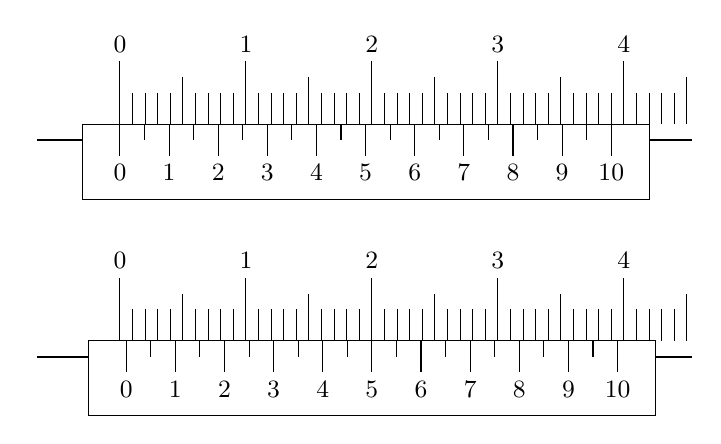
\begin{tikzpicture}%
  \node at (0, 0) {};
  \pgfmathsetmacro{\xscale}{0.16}
  \pgfmathsetmacro{\xstart}{30.}
  \pgfmathsetmacro{\y}{0.}
  
  {\small
  % Main scale.
  \draw[thick] (0,\y) -- (52*\xscale,\y);
  \foreach \x in {0,1,...,45}
  \draw[xshift=\xstart] (\x*\xscale,\y+0.2) -- (\x*\xscale,\y+0.6) {};
  \foreach \x in {0,5,...,45}
  \draw[xshift=\xstart] (\x*\xscale,\y+0.2) -- (\x*\xscale,\y+0.8) {};
  \foreach \x in {0,10,...,45}
  \draw[xshift=\xstart] (\x*\xscale,\y+0.2) -- (\x*\xscale,\y+1.0) node[anchor=south] {\pgfmathparse{0.1*\x}\pgfmathprintnumber{\pgfmathresult}};

  % Vernier scale
  \draw [fill=white,xshift=\xstart] (-3*\xscale,\y+0.2) rectangle (42*\xscale,\y-0.75);
  \foreach \x in {0,1,...,20}
  \draw[xshift=\xstart] (1.95*\x*\xscale,\y+0.2) -- (1.95*\x*\xscale,\y-0.) {};
  \foreach \x in {0,2,...,20}
  \draw[xshift=\xstart] (1.95*\x*\xscale,\y+0.2) -- (1.95*\x*\xscale,\y-0.2) node[anchor=north] {\pgfmathparse{0.5*\x}\pgfmathprintnumber{\pgfmathresult}};

  \pgfmathsetmacro{\y}{-2.75}

  % Main scale.
  \draw[thick] (0,\y) -- (52*\xscale,\y);
  \foreach \x in {0,1,...,45}
  \draw[xshift=\xstart] (\x*\xscale,\y+0.2) -- (\x*\xscale,\y+0.6) {};
  \foreach \x in {0,5,...,45}
  \draw[xshift=\xstart] (\x*\xscale,\y+0.2) -- (\x*\xscale,\y+0.8) {};
  \foreach \x in {0,10,...,45}
  \draw[xshift=\xstart] (\x*\xscale,\y+0.2) -- (\x*\xscale,\y+1.0) node[anchor=south] {\pgfmathparse{0.1*\x}\pgfmathprintnumber{\pgfmathresult}};

  % Vernier scale
  \draw [fill=white,xshift=\xstart] (-3*\xscale+0.5*\xscale,\y+0.2) rectangle (42*\xscale+0.5*\xscale,\y-0.75);
  \foreach \x in {0,1,...,20}
  \draw[xshift=\xstart] (1.95*\x*\xscale+0.5*\xscale,\y+0.2) -- (1.95*\x*\xscale+0.5*\xscale,\y-0.) {};
  \foreach \x in {0,2,...,20}
  \draw[xshift=\xstart] (1.95*\x*\xscale+0.5*\xscale,\y+0.2) -- (1.95*\x*\xscale+0.5*\xscale,\y-0.2) node[anchor=north] {\pgfmathparse{0.5*\x}\pgfmathprintnumber{\pgfmathresult}};
  }
\end{tikzpicture}
}{
    \caption{Illustrazione del funzionamento del nonio. Quando lo zero del nonio
      coincide con lo zero della scala principale (figura in alto), tutte le
      altre tacche del nonio sono disallineate rispetto a quelle della scala
      principale. Se spostiamo il nonio di mezzo~mm (figura in basso), l'unica
      tacca del nonio stesso a coincidere con una della scala principale
      è quella marcata con $5$ (decimi di~mm).}
    \label{fig:nonio}
  }
\end{figure}

Quando il calibro è \emph{chiuso} (cioè i becchi esterni sono a contatto
tra loro), lo zero del nonio corrisponde con lo zero della scala principale; di
conseguenza la ventunesima tacca del nonio (che è di nuovo marcata con uno
zero) coincide con la tacca dei $39$~mm della scala principale, mentre tutte le
altre divisioni del nonio saranno per definizione disallineate con le divisioni
della scala principale. Per inciso, questo è sempre vero: vi è al più
(e sempre, entro la risoluzione limitata del nostro occhio) una tacca del nonio
(o due, la prima e la ventunesima, nel caso dello zero) che coincide con una
tacca della scala principale.
Fino a qui tutto facile, ma adesso viene la parte interessante. Se spostiamo il
nonio di~$\nicefrac{1}{20}$~mm verso destra, la tacca dello zero sarà
leggermente disallineata con lo zero della scala principale.
La prima tacca del nonio a destra dello zero disterà
$\nicefrac{1}{20} + \nicefrac{39}{20} = 2$~mm dallo zero della scala principale
e coinciderà quindi con la tacca dei $2$~mm della scala stessa (tutte le
altre tacche del nonio, come sappiamo, saranno disallineate con la scala
principale). Se ci spostiamo ancora di $\nicefrac{1}{20}$~mm, la seconda tacca
del nonio a destra dello zero disterà dallo zero stesso 
$\nicefrac{2}{20} + 2 \times \nicefrac{39}{20} = 4$~mm e così via.
In assenza di errori di lettura la risoluzione del calibro appena descritto
è dunque $\nicefrac{1}{20}$~mm, da cui il nome di \emph{calibro ventesimale}.


\subsection{Lettura del calibro}

La tecnica di lettura del calibro si basa sul principio di funzionamento del
nonio illustrato brevemente nella sezione precedente e, come illustrato in
figura~\ref{fig:lettura_calibro}, si può riassumere nelle due semplici regole
che seguono:
\begin{enumerate}
\item la tacca della scala principale immediatamente inferiore allo zero del
  nonio indica la parte intera della lettura in~mm;
\item l'unica tacca del nonio che coincide con una (qualsiasi) delle tacche
  della scala principale indica la parte decimale della lettura e si
  legge direttamente dal nonio stesso in decimi di~mm.
\end{enumerate}


\begin{figure}[!htbp]
  \autohstack{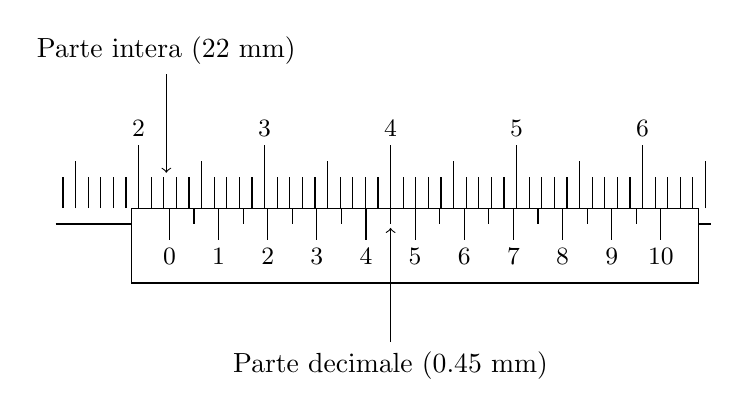
\begin{tikzpicture}%
  \node at (0, 0) {};
  \pgfmathsetmacro{\xscale}{0.16}
  \pgfmathsetmacro{\xstart}{30.}
  \pgfmathsetmacro{\y}{0.}
  {\small
  % Main scale.
  \draw[thick] (0,\y) -- (52*\xscale,\y);
  \foreach \x in {-6,-5,...,45}
  \draw[xshift=\xstart] (\x*\xscale,\y+0.2) -- (\x*\xscale,\y+0.6) {};
  \foreach \x in {-5,0,...,45}
  \draw[xshift=\xstart] (\x*\xscale,\y+0.2) -- (\x*\xscale,\y+0.8) {};
  \foreach \x in {0,10,...,45}
  \draw[xshift=\xstart] (\x*\xscale,\y+0.2) -- (\x*\xscale,\y+1.0) node[anchor=south] {\pgfmathparse{0.1*\x + 2}\pgfmathprintnumber{\pgfmathresult}};

  % Vernier scale
  \draw [fill=white,xshift=\xstart] (-3*\xscale+2.45*\xscale,\y+0.2) rectangle (42*\xscale+2.45*\xscale,\y-0.75);
  \foreach \x in {0,1,...,20}
  \draw[xshift=\xstart] (1.95*\x*\xscale+2.45*\xscale,\y+0.2) -- (1.95*\x*\xscale+2.45*\xscale,\y-0.) {};
  \foreach \x in {0,2,...,20}
  \draw[xshift=\xstart] (1.95*\x*\xscale+2.45*\xscale,\y+0.2) -- (1.95*\x*\xscale+2.45*\xscale,\y-0.2) node[anchor=north] {\pgfmathparse{0.5*\x}\pgfmathprintnumber{\pgfmathresult}};
  }

  \node[xshift=\xstart] (intera) at (2.2*\xscale,\y+2.2) {Parte intera ($22$~mm)};
  \draw[xshift=\xstart] [out=-90,in=90,-{>[scale=1.8]}] (intera) to (2.2*\xscale,\y+0.65);
  \node[xshift=\xstart] (decimale) at (1.95*9*\xscale+2.45*\xscale,\y-1.8) {Parte decimale ($0.45$~mm)};
  \draw[xshift=\xstart] [out=90,in=-90,-{>[scale=1.8]}] (decimale) to (1.95*9*\xscale+2.45*\xscale,\y-0.05);

\end{tikzpicture}
}{
    \caption{Esempio di lettura del calibro ventesimale. La parte intera si
      legge sulla scala principale e corrisponde alla prima tacca a sinistra
      dello zero del nonio---in questo caso $22$~mm. La parte decimale si
      legge sul nonio e corrisponde all'unica tacca che coincide con una della
      tacche della scala principale---in questo caso $\nicefrac{4.5}{10}$~mm.
      La lettura completa è dunque $22.45 \pm 0.05$~mm.}
    \label{fig:lettura_calibro}
  }
\end{figure}


\section{Il micrometro Palmer}

Il micrometro Palmer è uno strumento di misura della lunghezza con
risoluzione pari ad $\nicefrac{1}{100}$~mm. Il principio di funzionamento si
basa sull'avanzamento di una vite micrometrica che spinge un cilindro mobile
contro uno fisso---con l'oggetto da misurare posto tra i due come mostrato
in figura~\ref{fig:micrometro}. L'idea di base è che se il passo della vite
è abbastanza piccolo ed il suo diametro abbastanza grande, allora distanze
relativamente piccole possono essere \emph{amplificate} in rotazioni che possono
essere facilmente lette su una scala.

\medskip

\begin{figure}[!htbp]
  \centering
  \def\svgwidth{0.75\columnwidth}
  \input{figures/palmer_micrometer.pdf_tex}
  
  \caption{Esempio di lettura di un micrometro Palmer. In questo caso
    particolare l'ultima tacca visibile sul cilindro fisso è quella che
    corrisponde a $7.5$~mm---cui vanno aggiunti $0.17$~mm corrispondenti alla
    rotazione della parte mobile. La lettura sarà dunque $7.67 \pm 0.01$~mm.
    (Figura adattata
    da~\url{https://commons.wikimedia.org/wiki/File:Lecture_micrometre.svg}.)}
  \label{fig:micrometro}
\end{figure}


\subsection{Lettura del calibro Palmer e consigli pratici}

La lettura del calibro Palmer è semplice. Un giro completo del cilindro mobile
corrisponde ad una escursione lineare di $0.5$~mm e, corrispondentemente, il
cilindro fisso è graduato con una scala di uguale passo. La lettura si fa
dunque, al livello del mezzo millimetro, contando le tacche visibili sul
cilindro fisso. A questa va aggiunta la frazione di mezzo millimetro
corrispondente alla rotazione addizionale delle ghiera mobile, che è a sua
volta suddivisa in $50$ parti, come illustrato in figura~\ref{fig:micrometro}.

Data la risoluzione spinta (per un dispositivo puramente meccanico), è
necessario fare attenzione al momento torcente applicato nel processo di
misura---che, se troppo grande, potrebbe deformare l'oggetto da misurare, oltre
a danneggiare il calibro. A questo scopo i calibri Palmer sono tipicamente
dotati di un meccanismo di frizione, ed \emph{è sempre dalla frizione
  (anziché dalla ghiera graduata) che bisogna avvitare il tamburo}.

\`E buona norma controllare sempre che, quando il tamburo è completamente
avvitato, lo zero della ghiera corrisponda con l'asse graduato sul cilindro
fisso. Se così non è, allora si ha un problema di zero che si può
facilmente correggere per sottrazione alla fine della misura (o ricalibrando
opportunamente il dispositivo).

\`E utile notare, infine, come in pratica sia semplice (per errore di lettura
o imperfetta calibrazione dello strumento) sbagliare il conteggio delle
tacche sul cilindro fisso---che corrisponde a sbagliare la letture di $0.5$~mm,
o cinquanta volte la risoluzione del calibro. Per questo motivo è buona norma
ricontrollare le misure fatte con il calibro Palmer con un calibro ventesimale
che, pur avendo una risoluzione inferiore, può mettere in luce facilmente
eventuali errori grossolani.

